\documentclass[review]{elsarticle}

\usepackage{lineno,hyperref}
\modulolinenumbers[5]

\journal{Biomedical Signal Processing and Control}

%%%%%%%%%%%%%%%%%%%%%%%
%% Elsevier bibliography styles
%%%%%%%%%%%%%%%%%%%%%%%
%% To change the style, put a % in front of the second line of the current style and
%% remove the % from the second line of the style you would like to use.
%%%%%%%%%%%%%%%%%%%%%%%

%% Numbered
%\bibliographystyle{model1-num-names}

%% Numbered without titles
%\bibliographystyle{model1a-num-names}

%% Harvard
%\bibliographystyle{model2-names.bst}\biboptions{authoryear}

%% Vancouver numbered
%\usepackage{numcompress}\bibliographystyle{model3-num-names}

%% Vancouver name/year
%\usepackage{numcompress}\bibliographystyle{model4-names}\biboptions{authoryear}

%% APA style
%\bibliographystyle{model5-names}\biboptions{authoryear}

%% AMA style
%\usepackage{numcompress}\bibliographystyle{model6-num-names}

\usepackage{amsmath}
\usepackage{amsfonts}
\usepackage{amssymb}

%% `Elsevier LaTeX' style
\bibliographystyle{elsarticle-num}
%%%%%%%%%%%%%%%%%%%%%%%

\begin{document}

\begin{frontmatter}

\title{Capturing Waveforms in Polysomnography}

%% Group authors per affiliation:
\author{Giulia Carbonari\corref{mycorrespondingauthor}}
\author{Rodrigo Ramele}
\author{Juan Miguel Santos}
\author{Cecilia Forcato}
\address{Instituto Tecnológico de Buenos Aires}

%% or include affiliations in footnotes:
%\author[mymainaddress,mysecondaryaddress]{Elsevier Inc}
%\ead[url]{www.elsevier.com}

%\author[mysecondaryaddress]{Global Customer Service\corref{mycorrespondingauthor}}
\cortext[mycorrespondingauthor]{Corresponding author}
\ead{rramele@itba.edu.ar}

%\address[mymainaddress]{1600 John F Kennedy Boulevard, Philadelphia}
%\address[mysecondaryaddress]{360 Park Avenue South, New York}

\begin{abstract}
Winter cityside, crystal bits of snowflakes all around my head in the wind, I had no illusions that I've ever find the glimpse of summer heatwaves in your eyes. You did what you did it to me now its history i can see here's my comeback on the road again, things will happen when they can, I will wait here for my man tonight, its easy when you are Big In Japan.
Neon on my naked skin, passing silhouettes of strange illuminated mannequins, shall i stay here at the zoo, or shall i go to change my point of view for other ugly scene.
\end{abstract}

\begin{keyword}
SIFT, EEG, waveform
%\MSC[2010] 00-01\sep  99-00
\end{keyword}

\end{frontmatter}

\linenumbers

\section{Introduction}

Bidimensional images can be interpreted as bidimensional signals.   Instead of having amplitude values for a time series, they can be interpreted as having amplitude values for two varying independent variables (height and width).

This method proposed a different approach, where EEG signals are studied based on the shape of their waveforms, graphoelements that conceive cognitive meaning, or that represent medical conditions.  Having such a method, allows a mapping quantitive mapping of EEG signals and components which at the same time conceive meaning to the practicioners clinician, technician or physician that is studying these signals.  Like a common language.

This work  expands the method presented here, here and here.  It establishes their modeling and extend their usage to the study of polysomnographic signals, which are particularly suitable to be analyzed in this way.

This work unfolds as follows.  The first section provides the general layout of the model.  Section II presents a brief section and an accompanying software that can be used to obtain descriptors from images and that can be integrated into other projects to perform this analysis.  For the experiment section we analyzed a database of Sleep Research, and in the Results section we proved how this method can be used to identify slow waves.   Conclusions and future research directions are outlined in the last section.

\section{Converting images}

Once the regularization procedure,  the size and the scale of the image are defined,  a binary image $\mathcal{I}^{(c)}$ can be constructed from a variant of the method specified in Equation~\ref{eq:image1} according to

\begin{equation}
\mathcal{I}^{(c)}(z_1,z_2) = \left\{ \begin{array}{rl}
255 & \text{if} \   z_1 = \gamma_{t} \  n \quad \text{and}  \quad z_2 = \left\lfloor \gamma \; \tilde{x}(n,c) \right\rceil + z(c) \\
0   & \mbox{otherwise}
\end{array}\right.
\label{eq:images}
\end{equation}

\noindent  where  $1 \leq c \leq C$ and $1 \leq n \leq N$. The amplitude scale factor $\gamma$ and time scale factor $\gamma_{t}$ are used to determine the image size and at the same time the image resolution. This scheme produces a black-and-white plot of the signal with $255$ being white and $0$ black.  There is one image per channel per segment. 

%\noindent with $255$ being white and representing the signal's voltage in relation to the zero-level $z(c)$, and $0$ for black which is the background contrast. This scheme produces a black-and-white plot of the signal.  Pixel arguments $ (z_1,z_2) \in \mathbb{N} \times \mathbb{N}$ iterate over the width $\gls{Wx}$ and height $\gls{Hy}$  of the image plot with $1 \leq n \leq N$ and $1 \leq c \leq C$.  There is one image per channel.  The parameters $\gamma$ and $\gamma_t$ are the amplitude and time scaling factors.  They are used to determine the image size and at the same time the image resolution.

\paragraph{A Digitalization Procedure} 

\paragraph{Resolution and Precision} 



\section{The SIFT: Histogram of Gradient Orientations}
\label{SIFT}


The basic procedure is composed of,

\begin{enumerate}
\item Keypoints $kp$ are located on an image of a signal plot.
\item A region of an image, a patch, is established using keypoints as centers.  Each patch has a horizontal $St$ and vertical scale $Sv$, which determines the size in pixels $Sx$ and $Sy$,  along the horizontal and vertical axis respectively. 
\item From each patch, a descriptor $d$ is derived which is used as a representation of the graphical information contained within the patch.
\end{enumerate}

On the image generated by the procedure detailed in previous Chapter, a keypoint $kp$ is placed on a pixel $(x_{kp}, y_{kp})$ over the image plot and a window around the keypoint is considered. A local image patch of size $Sx \times Sy$ pixels is constructed by dividing the window in $16$ blocks. It is arranged in a $4 \times 4$ grid and the pixel $kp$ is the patch center.  Figure~\ref{fig:sampledescriptor}(a) shows a plot of a signal, a keypoint in red at the center and the surrounding patch.

Pixel intensity gradients can be obtained from an image by applying the Sobel filter~\cite{Szeliski2010} and using finite differences to obtain pixel differences on the $x$ and $y$ direction.  Composing them as vectors, oriented gradients on each pixel can be calculated.  Figure~\ref{fig:sampledescriptor}(b) and (c) show vector field of oriented gradients.

A local representation of the signal shape within the patch can be described by obtaining the gradient orientations on each of the $16$ blocks and creating a histogram of gradients.  In order to calculate the histogram, the interval $[0-360]$ of possible angles is divided in $8$ bins, each one at $45$ degrees.  Figure~\ref{fig:sampledescriptor}(d) shows a sample histogram obtained for eight orientations.

Hence, for each spatial bin $ i,j = \{0,1,2,3\} $, corresponding to the indexes of each block $B_{i,j}$,  the orientations are accumulated in a  $3$-dimensional histogram $h$ through the following equation: 
 

\begin{equation}
 h(\theta,i,j) = \sum_{\mathbf{p}} \omega_\mathrm{ang}(\angle J(\mathbf{p}) - \theta)\, \omega_{ij}\left(\mathbf{p} - \mathbf{kp} \right)\, \left\lVert J(\mathbf{p})\right\rVert 
\label{eq:histogram}
\end{equation}

\noindent  where $\mathbf{p}$ is a pixel from within the patch,  $\theta$ is the angle bin with $ \theta \in \{0, 45, 90, 135, 180, 225, 270, 315\} $,  $ \left\lVert J(\mathbf{p}) \right\rVert $ is the norm of the gradient vector in the pixel $\mathbf{p}$, computed using finite differences, and $\angle J(\mathbf{p}) $ is the angle of the gradient vector.  The scalar $ \omega_\mathrm{ang}(\cdot) $  and vector $ \omega_{ij}(\cdot) $ functions are linear interpolations used by~\cite{Lowe2004} and \cite{Vedaldi2010} to provide a weighting contribution to eight adjacent bins.  They are calculated as  

\begin{equation}
 \omega_{ij}(\mathbf{v}) = \omega \bigg ( \frac{5 \;v_x}{\Delta s \; St} - x_i \bigg ) \omega \bigg ( \frac{5 \; v_y}{\Delta s \; Sv} - y_i \bigg ) 
\label{eq:ij}
\end{equation}

\begin{equation}
 \omega_\mathrm{ang}(\alpha) = \sum_{r=-1}^{1} \omega \bigg ( \frac{8\alpha}{2\pi} + 8r \bigg )
\label{eq:wang}
\end{equation}

\noindent where $x_i$ and $y_i$ are the spatial bin centers located in $ x_i,y_i \in \{-\frac{3}{2},-\frac{1}{2},\frac{1}{2},\frac{3}{2}\} $. The function parameter $\mathbf{v} = ( v_x, v_y ) $ is a vector variable and $\alpha$ a scalar variable.  The value of  $\Delta s$ is the unit length of the patch, which is described in the section~\ref{patchgeometry}.  On the other hand, $r$ is an integer that can vary freely in the set $\{ -1, 0, 1 \} $ and allows the argument $\alpha$ to be unconstrained in terms of its values in radians. The interpolating function $\omega(\cdot)$ is defined as:

\begin{equation}
\omega(z) = \max(0,1-|z|).
\label{eq:weighting}
\end{equation}

These binning functions conform a trilinear interpolation that has a combined effect of sharing the contribution of each oriented gradient between their eight adjacent bins in a tridimensional cube in the histogram space, and zero everywhere else.  This procedure is important to avoid quantization issues that may appear with the histogram (i.e. elimination of intermediate values).

Lastly, on Equation~\ref{eq:ij} the values of $ \frac{5}{\Delta s \; St} $ and $ \frac{5}{\Delta s \; Sv} $ allow a unit conversion from pixel to units-of-patch.  As the patch has  $16$ blocks and  $8$ bin angles are considered, a feature $d$ called \textit{descriptor} of $128$ dimension is obtained. This technique is a modification of Lowe's SIFT Descriptor method.

In Figure~\ref{fig:orientationsfull} the possible orientations on each patch are illustrated.  The first eight orientations of the first block $ B_{1,1} $, are labeled from $1$ to $8$ clockwise. The orientations of the second block $ B_{1,2} $ are labeled from $9$ to $16$.  This labeling continues left-to-right, up-down until the eight orientations for all the sixteen blocks are assigned. They form the corresponding $\mathbf{kp}$-descriptor of $128$ coordinates.


\begin{figure}[h!]
\centering
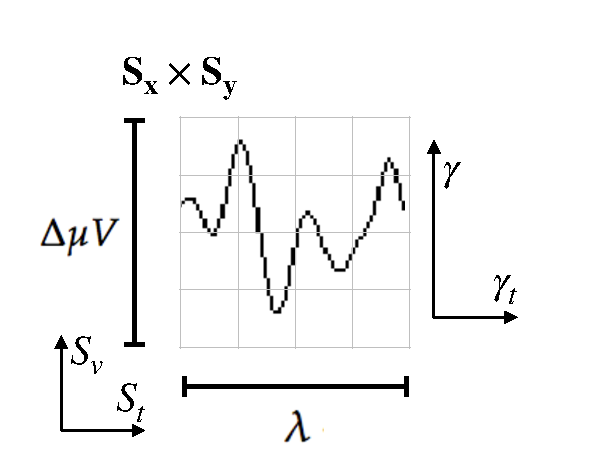
\includegraphics[width=10cm]{images/patchgeometry.pdf}
\caption[Patch Geometry]{  }
\label{fig:patchgeometry}
\end{figure}

\paragraph{Installation} If the document class \emph{elsarticle} is not available on your computer, you can download and install the system package \emph{texlive-publishers} (Linux) or install the \LaTeX\ package \emph{elsarticle} using the package manager of your \TeX\ installation, which is typically \TeX\ Live or Mik\TeX.

\paragraph{Usage} Once the package is properly installed, you can use the document class \emph{elsarticle} to create a manuscript. Please make sure that your manuscript follows the guidelines in the Guide for Authors of the relevant journal. It is not necessary to typeset your manuscript in exactly the same way as an article, unless you are submitting to a camera-ready copy (CRC) journal.

\paragraph{Functionality} The Elsevier article class is based on the standard article class and supports almost all of the functionality of that class. In addition, it features commands and options to format the
\begin{itemize}
\item document style
\item baselineskip
\item front matter
\item keywords and MSC codes
\item theorems, definitions and proofs
\item lables of enumerations
\item citation style and labeling.
\end{itemize}

Here are two sample references: \cite{Feynman1963118,Dirac1953888}.

\section{Mapping between Signal Features and Patch Descriptor}

\section{Slow Wave and KComplex identification}

Sleep Research is devoted to understand the inner workings of the brain during sleep and its strong connection with memory.  The traditional approach to glimpse what is happening inside the brain while sleeping has been the Electroencephalography, which received a particular term when it is used for this purpose: Polysomnography (PSG).  Sleep research studies rely heavily on EEG graphoelements (CITE) like K-Complexes, Slow Waves, and they are key components used to determine sleep stage. BLA BLA BLA

This makes PSG signal analysis particular relevant for this methodology, because it can be used to derive a metric that can describe quantitative the similarities between signal shape components.  Sleep research requires long hours of data analysis hence, it will benefit from automation tools that at the same speak the same language than those who traditionally analyze these signals.

BLA BLA BLA

\paragraph{Dataset}

The dataset used is THIS.  It contains EEG data for 10 subjects.  More information can be obtained from HERE.


\section*{References}

\bibliography{sift}

\end{document}
